\chapter{Literature Review}

\section{History of Nuclear Fuel Cycle Simulators}
The nuclear fuel cycle represents the life cycle of nuclear fuel from initial
extraction, processing, use in reactors, and, eventually, 
final disposal.
It is a complex system of facilities and mass flows 
that are combined to meet the goal of providing nuclear energy 
in the form of electricity \cite{yacout_modeling_2005}.
A closed \gls{NFC} reprocesses used fuel, whereas an open 
\gls{NFC} does not.  
The US has an open \gls{NFC}; other countries, such as France, 
have a closed NFC. 

\gls{NFC} simulators are system analysis tools used to evaluate 
quantitative measures of dynamic \gls{NFC} performance 
in both high and low resolution. 
Plutonium concentration in a single used fuel bundle and 
total electricity produced are examples of high and low 
resolution elements, respectively.   
The primary purpose of \gls{NFC} simulators is to understand the 
dependence between various input parameters and components 
in the \gls{NFC} and the impact their variations have on 
the system's performance. 
The results of \gls{NFC} simulators are used to guide research 
efforts, advise future design choices, and provide 
decision-makers with a transparent tool for evaluating \gls{FCO} 
to inform big-picture policy decisions \cite{yacout_modeling_2005}.

% Where are NFC codes from 
Historically, national laboratories around the globe have driven 
development and are the primary users of \gls{NFC} simulator tools. 
However, due to propriety access to these tools, universities and 
other non-laboratory organizations have taken to creating their 
own \gls{NFC} simulator tools. 
Table \ref{tab:nfctools} shows a breakdown of all major \gls{NFC} simulators
and the organization(s) associated with them.  

\begin{table}[]
    \centering
    \footnotesize
    \begin{tabular}{ll}
    \hline
    \textbf{\gls{NFC} simulator} & \textbf{Organization(s) associated with it}                                    \\ \hline
    \Cyclus \cite{huff_fundamental_2016}                & \gls{UW}, \\ & \gls{UIUC} \\ 
    DYMOND \cite{yacout_modeling_2005},                                & \gls{ANL}                                                                                               \\ 
    ORION  \cite{gregg_analysis_2012}                                & \gls{NNL}                                                                                             \\ 
    VISION \cite{jacobson_vision:_2006}                                & \gls{INL}                                                                                               \\ 
    COSI   \cite{coquelet-pascal_cosi6:_2015}                                &   \gls{CEA}                    \\ 
    CLASS  \cite{mouginot_class_2012}                                &  \gls{CNRS}, \\ & \gls{IRSN}                                    \\
    DESAE  \cite{tsibulskiy_desae_2006} & \gls{OECD} \\ \hline
    \end{tabular}%
    \caption{Nuclear Fuel Cycle Simulator Tools and their corresponding organizations.}
    \label{tab:nfctools}
    \end{table}

% what is agent, what is fleet
There are two methods to model facility and material flow in 
\gls{NFC} simulators: fleet-level and agent-level.  
Fleet-based models do not distinguish between discrete facilities 
or materials but instead lumps them into fleets and streams. 
The advantages of this method are a more straightforward code 
structure and lower computational cost.
Agent-based models treat facilities and materials as discrete 
objects. 
The advantages of this method are more flexible simulation control
and ease of simulating a wide range of scenarios with new 
technologies.  

% why is it good that there are multiple tools 
% benchmark against each other
The U.S. national laboratories conducted a benchmarking effort to 
verify NFC simulators against each other
\cite{feng_standardized_2016,guerin_benchmark_2009}. 
These comparison studies assist developers in improving the
codes to more realistically model the \gls{NFC}. 
Furthermore, by upholding the \gls{NFC} simulator tools to 
a high level of agreement, 
stakeholders and decision-makers can have more confidence in 
prediction results generated by \gls{NFC} simulator tools and trust them 
to inform on potential strategic and policy decisions
\cite{feng_standardized_2016}. 

\section{Transition Scenarios}
Chapter 1 gave an overview of the history and motivation of 
\gls{NFC} transition scenario research.
This section gives a more detailed description of the motivation 
behind transition scenario studies.
The evaluation and screening study identified 40 promising 
evaluation groups (\glspl{EG}) to represent a comprehensive set of 
fuel cycle options (\gls{FCO}) \cite{wigeland_nuclear_2014}. 
The study conducted an assessment of each EG using 
9 evaluation criteria: nuclear waste management, 
proliferation risk, nuclear material security risk, 
safety, environmental impact, resource utilization, 
development and deployment risk, institutional issues, and 
financial risk.  
The study concluded that fuel cycles
involving continuous recycling of co-extracted U/Pu or U/TRU in 
fast spectrum critical reactors consistently scored high overall 
performance.
EG23, EG24, EG29, and EG30 are the high-performing fuel cycle options.
Table \ref{tab:eg} describes the current US EG
and the high-performing \glspl{EG}. 
These \glspl{EG} were evaluated at an equilibrium state to 
understand their end-state benefits.
Knowing the most promising end-state \glspl{EG}, 
the next step is to evaluate and compare the transition process 
from the current EG01 
state to these promising \glspl{EG} \cite{feng_standardized_2016}. 

\begin{table}[]
    \centering
    \caption{Descriptions of the current and other high performing nuclear fuel cycle evaluation groups described in the evaluation and screening study \cite{wigeland_nuclear_2014}.}
    \label{tab:eg}
        \footnotesize
        \begin{tabular}{llll}
            \hline
        \textbf{Fuel Cycle}                                               & \textbf{Open or Closed} & \textbf{Fuel Type}                                                              & \textbf{Reactor Type}                                                                           \\ \hline
        \textbf{\begin{tabular}[c]{@{}l@{}}EG01\\ (current)\end{tabular}} & Open                                                               & Enriched-U                                                                      & Thermal Critical                                                                       \\ 
        \textbf{EG23}                                                     & Closed                                                             & \begin{tabular}[c]{@{}l@{}}Recycled U/Pu \\ + Natural-U\end{tabular}  & Fast Critical                                                                         \\ 
        \textbf{EG24}                                                     & Closed                                                             & \begin{tabular}[c]{@{}l@{}}Recycled U/TRU \\ + Natural-U\end{tabular} & Fast Critical                                                                   \\ 
        \textbf{EG29}                                                     & Closed                                                             & \begin{tabular}[c]{@{}l@{}}Recycled U/Pu \\ + Natural-U\end{tabular}  & Fast Critical \& Thermal Critical  \\ 
        \textbf{EG30} & Closed                                                             & \begin{tabular}[c]{@{}l@{}}Recycled U/TRU \\ + Natural-U\end{tabular} & Fast Critical \& Thermal Critical  \\ \hline
    \end{tabular}
\end{table}

\section{\gls{NFC} simulators Transition Scenario Capabilities}
% what has been done for transition scenarios so far
Both \gls{NFC} simulator tools used in this thesis, \Cyclus and DYMOND,
were verified in a transition scenario benchmarking effort
\cite{feng_standardized_2016,bae_standardized_2019}.
The reference problem used in the benchmark was a simplified 
transition of one hundred 1000-MWe \glspl{LWR} to a fleet 
of 333.3-MWe \gls{SFR} fleet. 
They were found to have excellent agreement with the 
spreadsheet solution and other \gls{NFC} codes.  
This benchmarking effort proved that these \gls{NFC} simulators
are capable of simulating a simple transition scenario. 
However, it acknowledged that there needs to be more efforts 
made to model realistic transition scenarios to evaluate the
flexibility of the \gls{NFC} simulators \cite{feng_standardized_2016}.
Chapter \ref{chap:3} gives in-depth descriptions of \Cyclus and DYMOND.

\section{\gls{NFC} simulators Sensitivity Analysis}
We simulate transition scenarios to predict the future; 
however, when implemented in the real world, they tend to deviate 
from the optimal scenario.
Therefore, \gls{NFC} simulators must be used to conduct
sensitivity analysis studies to understand the nuances of 
a transition scenario better to inform policy decisions reliably
\cite{passerini_systematic_2014}. 

Previous work towards Sensitivity Analysis (SA) and \gls{UQ} of 
\gls{NFC} simulations used these terms interchangeably
because \gls{UQ} is viewed as design uncertainty.
For example, a never-been-built pyrochemical reprocessing 
facility's throughput is viewed as a design parameter that 
can be varied.
We determine the impact of the variation of the pyroprocessing 
facility's throughput on essential output parameters.
Similarly, by conducting studies on a more extensive set of input 
parameters, it is possible to determine the most sensitive input 
parameters.
This provides a target of where we should conduct closer 
sensitivity analysis and add further modeling detail.
It also identifies which parameters the system is relatively 
insensitive to \cite{noauthor_effects_2017}. 

\gls{SA} is a technique used to determine how the variation of 
different input variable(s) impacts the output of a given 
scenario. 
When setting up the simulation scenarios, many assumptions are made. 
\gls{SA} assists in the evaluation of the sensitivity of the 
output of the scenario to each of these assumptions. 
There are three types of sensitivity analysis: 
one-at-a-time (OAT), synergistic, and global.

\subsection{One-at-a-time Sensitivity Analysis}
OAT is a basic \gls{SA} technique that focuses on estimating 
the lone effect of one input variable. 
This approach gives the local impact of each variable on the 
output parameters of interest. 
OECD conducted an OAT sensitivity analysis \cite{noauthor_effects_2017} 
on key \gls{NFC} input parameters
and quantified the impacts on the selected output parameters. 
The base scenario used has a duration of 200 years and begins 
with a fleet of \glspl{PWR}, transitioning to \glspl{SFR} while 
maintaining constant electricity production. 
Each parameter was varied independently for three cases: 
the base case, a high case, and a low case (relative to the base 
case). 
The results of these variations on the output parameters 
are expressed in tornado plots and sensitivity tables. 
Figure \ref{fig:oecd-sensitivitytable} shows the sensitivity table
provided by the benchmark that gives an overview of their analysis. 
Figure \ref{fig:oecd-tornado} shows an example tornado plot that represents 
the sensitivity of separated Pu in storage to the various input parameters. 

\begin{figure}[]
	\begin{center}
		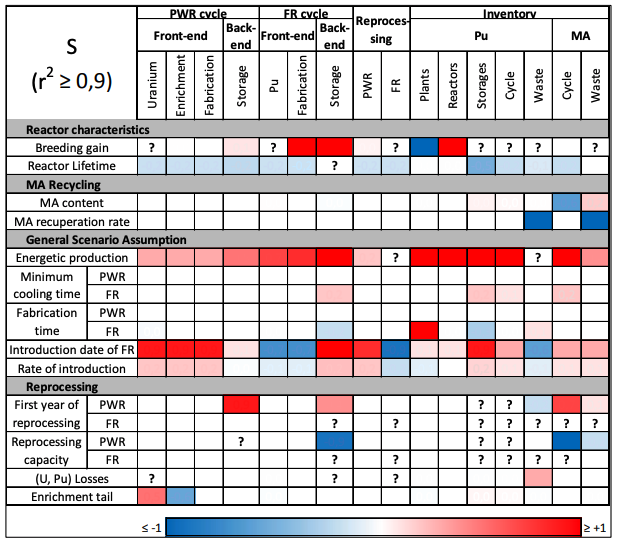
\includegraphics[scale=0.55]{./figures/oecd-sensitivitytable.png}
	\end{center}	
		\caption{Sensitivity Table that provides an overview of the sensitivity 
		of each output parameter to the respective input parameters \cite{noauthor_effects_2017}.}
	\label{fig:oecd-sensitivitytable}
\end{figure}

\begin{figure}[]
	\begin{center}
		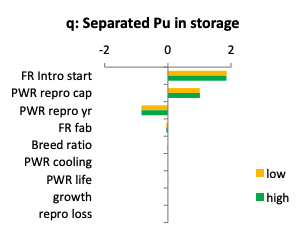
\includegraphics[scale=0.65]{./figures/oecd-tornado.png}
	\end{center}	
		\caption{Tornado plot showing the sensitivity of separated Pu in 
		storage to relation to each input parameter \cite{noauthor_effects_2017}.}
	\label{fig:oecd-tornado}
\end{figure}

\subsection{Synergistic Sensitivity Analysis}
The Synergistic \gls{SA} technique involves multi-parameter 
input sweeps to view the impact of synergistic 
changes of input variables on specific output variables. 
Synergistic \gls{SA} can be conducted by varying 
two input variables simultaneously and viewing their 
combined impact on each output parameter or a combination 
of weighted output parameters. 
Figure \ref{fig:passerini_payoff} shows an example of this analysis 
in which thermal reprocessing and fast reactor technology 
introduction dates were varied, and the plot shows an objective 
payoff surface representing a combination of multiple optimization 
criteria. 
This method of synergistic study informs on the local effects of 
two input variables on the system; however, it fails to inform 
on the global sensitivity of the system. 

\begin{figure}[]
	\begin{center}
		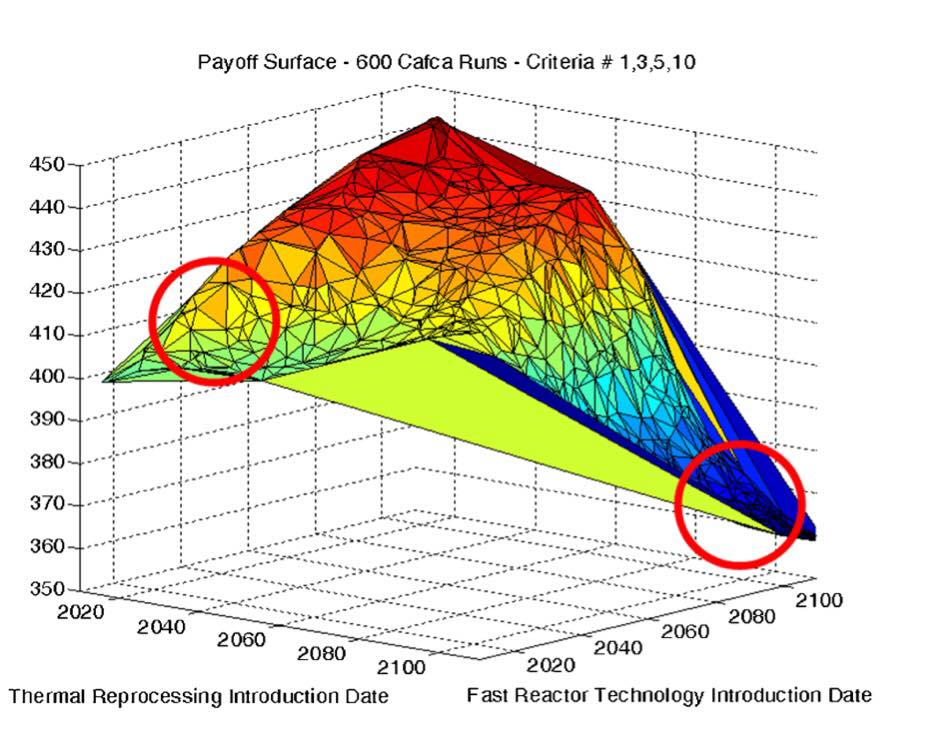
\includegraphics[scale=0.25]{./figures/passerini_payoff.jpg}
	\end{center}	
		\caption{Optimization Surface of the payoff when varying thermal 
		reprocessing and fast reactor technology introduction date
		\cite{passerini_systematic_2014}}
	\label{fig:passerini_payoff}
\end{figure} 

\subsection{Global Sensitivity Analysis}
\label{sec:sobol}
To fully consider the synergistic effects of
simultaneous variation of the input variables, a variance-based 
approach can be used instead \cite{thiolliere_methodology_2018}.
Thiolliere et al. conducted a global sensitivity analysis of a 
\gls{NFC} transition scenario by using Latin Hypercube sampling 
to generate Sobol indices. 
Sobol Indices provide the global sensitivity effect of each 
input variable by decomposing the variance of the output into 
fractions attributed to inputs or sets of inputs.
Essentially, it indicates which design parameter has 
the most influence on the response quantities.
A large Sobol indices value signifies that variation in that input 
variable is more impactful to the output parameter.

\subsection{Main Takeaways}
\gls{SA} studies of \glspl{NFC} have previously been used to narrow 
down and compare a wide range of \gls{NFC} scenarios to determine 
the ideal scenario end types. 
The evaluation and screening study determined that the desired 
fuel cycle end states were EG23, EG24, EG29, and EG30.
These \gls{SA} studies focused on high level input 
parameters such as reactor and reprocessing technologies, etc.
However, limited sensitivity studies have been performed to 
evaluate specific transition scenarios that describe the transition 
from the current to desired end states.
The only relevant sensitivity study was conducted by OECD 
\cite{noauthor_effects_2017}, however it was a basic OAT 
\gls{SA}.   
Therefore, synergistic \gls{SA} studies focused on
lower-level input parameters such as cooling time, 
date of introduction of reprocessing/reactor 
technologies, the ratio of technology types should be conducted to 
understand the nuances of the variation of these low-level parameters. 
Through synergistic \gls{SA}, these transition scenarios can be 
further optimized and used to inform other nuclear research areas 
such as reprocessing facility design, etc. 